% Магистерская диссертация Дворянкина В.В. (АСМ-24-04)
% Тема: «Разработка моделей и сервиса для интерактивного взаимодействия с обучающимися»
% Научный руководитель: Волков Д.А., к.т.н., доцент кафедры АСУ
% РГУ Нефти и Газа (НИУ) им. И.М. Губкина, 2026
%
% Шаблон: gitea.volkov.top/edu/edu-tex-template (Stulk3, ValeryVerkhoturov)

\documentclass[14pt, a4paper]{extarticle}

%%%%%%%%%%%% Пакеты %%%%%%%%%%%%%%%%%%
\usepackage{polyglossia} % языковой пакет

\usepackage{pdfpages} % пакет для импорта pdf-файлов

\usepackage{tocvsec2} %%%%%%%%%%%%%%%%%%%%%%%%%%%%%%%%%

% Подписи рисунков и таблиц по требованию кафедры АСУ:
% «Рисунок 1 — Описание», разделитель — длинное тире.
\usepackage[labelsep=endash]{caption}
% Polyglossia сбрасывает \figurename на «Рис.» при активации русского
% языка, поэтому \renewcommand{\figurename}{...} в преамбуле и даже
% \AtBeginDocument срабатывают ненадёжно. Самый прямой способ —
% задать имя метки в caption-пакете через name=..., минуя \figurename.
\captionsetup[table]    {name=Таблица, labelsep=endash, justification=raggedleft, singlelinecheck=off, position=above}
\captionsetup[figure]   {name=Рисунок, labelsep=endash, justification=centering,  singlelinecheck=on,  position=below}
\captionsetup[lstlisting]{labelsep=endash, justification=centering, singlelinecheck=on,  position=below}
% Дублируем через \AtBeginDocument для пакетов, читающих \figurename
% напрямую (например, hyperref для подписей якорей).
\AtBeginDocument{%
    \renewcommand{\figurename}{Рисунок}%
    \renewcommand{\tablename}{Таблица}%
}

\usepackage{titletoc}

% \usepackage{misccorr} отключён: пакет добавляет точку после номера
% в подписях рисунков/таблиц (делает «Рисунок 1.1.», «Таблица 1.1.»),
% что мешает применению нашего labelsep=endash. Точки в оглавлении
% и так формируются дотлидером \titlecontents, без misccorr.

\usepackage{graphicx} % пакет для использования графики (чтобы вставлять рисунки, фотографии и пр.)

\usepackage{amsmath} % поддержка математических символов

\usepackage{url} % поддержка url-ссылок

\usepackage{lipsum}

% Legacy команда \bibliographystyle{gost-numeric.bbx} удалена:
% biblatex + biber не используют bibtex'овский bibliographystyle.
% Минимальный набор опций ГОСТ-стиля; deprecated parentracker
% и проблемная пара defernumbers+sorting=none убраны — они вызывали
% Missing number в \printbibliography.
\usepackage[
    backend=biber,
    bibencoding=utf8,
    style=gost-numeric,
    language=auto,
    autolang=other,
    sorting=nty
]{biblatex}
% Принудительная сортировка: сначала русскоязычные источники,
% затем иностранные. Реализуется через поле presort в refs.bib:
% русские записи — presort={a}, латинские — presort={z}.
% При sorting=nty biber сортирует presort → name → year → title.
\addbibresource{refs.bib}

% Переопределение биб-локализации под ГОСТ Р 7.0.100-2018:
% - urlseen ('дата обращения' вместо biblatex-gost-дефолта 'дата обр.')
% - bibrangedash (короткое тире en dash в диапазонах страниц '23–31'
%   вместо длинного тире, которое biblatex-gost подставляет в русском
%   режиме).
\DefineBibliographyStrings{russian}{%
    urlseen = {дата обращения},
}
\AtBeginDocument{\def\bibrangedash{\textendash}}

\usepackage{fancyhdr} % заголовок

\usepackage{enumitem} % списки

\usepackage{multirow} % таблицы с объединенными строками

\usepackage{hyperref} % пакет для интеграции гиперссылок

\usepackage{indentfirst} % пакет для отступа абзаца


\usepackage{chngcntr} % пакет подписей и нумерации рисунков

\usepackage{setspace}

\usepackage{csquotes}

\usepackage{tabularx}

% Альбомная ориентация для широких диаграмм (use case, flowchart).
\usepackage{pdflscape}
\usepackage{rotating}

% Барьер для плавающих объектов (рисунков и таблиц): \FloatBarrier
% не позволяет рисунку «уплывать» в следующий подраздел.
\usepackage{placeins}
% Пакет float даёт спецификатор [H] для строгой фиксации рисунка
% в указанном месте — используется в макросе \imageH (без float).
\usepackage{float}

% Эмуляция пакета needspace (пакет в TL2026 basic недоступен
% без прав администратора). \needspace{N\baselineskip} ломает
% страницу, если на текущей странице осталось места меньше N.
% Используется для предотвращения висячих заголовков перед
% подразделами и листингами в приложениях.
\makeatletter
\providecommand\needspace[1]{%
    \par\penalty-100%
    \begingroup
        \dimen@\pagegoal
        \advance\dimen@-\pagetotal
        \ifdim\dimen@<#1\relax
            \pagebreak
        \fi
    \endgroup}
\makeatother

% Параметры выключки абзаца: уменьшаем «реки» пробелов в узких
% колонках русского текста за счёт более гибкого emergencystretch
% и более терпимого hyphenpenalty при выключке по ширине.
\tolerance=1000
\emergencystretch=3em
\hyphenpenalty=50

%%%%%%%%%%%%%%%%%%%%%%%%%%%%%%%%%%%%%%%%%%%%%%%%%%%%%%%%%%%%%%

%%%%%%%%%%%% Формат %%%%%%%%%%%%%%%%%%
%%%%%%%%%%%%%%%%% Оформление ГОСТА%%%%%%%%%%%%%%%%%

% Все параметры указаны в ГОСТЕ на 2021, а именно:

% Шрифт для курсовой Times New Roman, размер – 14 пт.
\setdefaultlanguage[spelling=modern]{russian}
    \setotherlanguage{english}

% Шрифты подключаются явно из ./fonts/ — независимо от системных установок,
% работает одинаково локально и в CI.
% Ligatures=TeX включает: --- → —, -- → –, `` → " и т.д.
\defaultfontfeatures{Path=fonts/, Ligatures=TeX}

\setmainfont{FontsFree-Net-times-new-roman.ttf}
\setromanfont{FontsFree-Net-times-new-roman.ttf}
\newfontfamily\cyrillicfont{FontsFree-Net-times-new-roman.ttf}

% Source Code Pro: загружаем Regular + Bold явно из файла.
% Italic-вариант файла — variable font; пропускаем, чтобы не падать
% на старых сборках TeX Live; курсив синтезируется fontspec'ом при необходимости.
\setmonofont{SourceCodePro-Regular.ttf}[
    BoldFont = SourceCodePro-Bold.ttf,
    AutoFakeSlant = 0.2,
]
\newfontfamily{\cyrillicfonttt}{SourceCodePro-Regular.ttf}[
    BoldFont = SourceCodePro-Bold.ttf,
    AutoFakeSlant = 0.2,
]




% шрифт для URL-ссылок
\urlstyle{same} 

% Междустрочный интервал должен быть равен 1.5 сантиметра.
\linespread{1.5} % междустрочный интервал


% Отступы списков по требованию кафедры:
% «Положение метки 1.25 см, положение текста 0» — метка-нумерация
% стоит как абзацный отступ, тело пункта (включая продолжающиеся
% строки) начинается с левого края страницы, как обычный абзац.
% Это эквивалент Word: «Отступ слева 0, отступ первой строки 1.25 см».
% В enumitem прямой синоним этого — опция wide=<dimen>: пункт
% оформляется как обычный параграф с отступом первой строки.
% Между пунктами — без дополнительного интервала; межстрочный 1.5
% наследуется от \linespread{1.5}.
\setlist[enumerate,1]{
    wide=1.25cm,
    label=\arabic*.,
    labelsep=0.5em,
    topsep=0pt, parsep=0pt, partopsep=0pt, itemsep=0pt,
}
\setlist[itemize,1]{
    wide=1.25cm,
    label=\textendash,
    labelsep=0.5em,
    topsep=0pt, parsep=0pt, partopsep=0pt, itemsep=0pt,
}
\setlist[itemize,2]{label=$\circ$, leftmargin=1cm}



% Каждая новая строка должна начинаться с отступа равного 1.25 сантиметра.
\setlength{\parindent}{1.25cm} % отступ для абзаца

% Текст, который является основным содержанием, должен быть выровнен по ширине по умолчанию включен из-за типа документа в main.tex


%%%%%%%%%%%%%%%%%% Дополнения %%%%%%%%%%%%%%%%%%%%%%%%%%%%%%%%%

% Пути до папок с изображениями
\graphicspath{ {./Images/}{./figures/} }

% Внесение titlepage в учёт счётчика страниц
\makeatletter
\renewenvironment{titlepage} {
	\thispagestyle{empty}
}


% Цвет гиперссылок и цитирования
\usepackage{hyperref} 
 \hypersetup{ 
     colorlinks=true, 
     linkcolor=black, 
     filecolor=blue, 
     citecolor = blue,       
     urlcolor=blue, 
     }
    

% Нумерация рисунков
%\counterwithin{figure}{section}
%\counterwithin{figure}

% Нумерация таблиц
%\counterwithin{table}

%\counterwithin{table}{section}

% шрифт для листингов с лигатурами
% \setmonofont{FiraCode-Regular.otf}[
% 	SizeFeatures={Size=10},
% 	Path = Settings/,
% 	Contextuals=Alternate
% ]
% \setmonofont уже задан выше (см. блок шрифтов с Path=fonts/).
% \setmonofont{Source Code Pro}

% Запрет переносов слов через дефис (по образцу кафедры АСУ).
% Текст «растягивается» межсловными пробелами вместо переноса.
\hyphenpenalty=10000
\exhyphenpenalty=10000
\sloppy
\tolerance=9999
\emergencystretch=4em

% Сквозная нумерация рисунков, таблиц, формул, листингов (по требованиям кафедры).
% При желании заменить на двухуровневую: \counterwithin{figure}{section} и т.д.
% Сейчас оставляем сквозную --- она проще для отслеживания ссылок.

% Запрет на висячие строки (orphans) и заголовков, оторванных от текста (widows).
\widowpenalty=10000
\clubpenalty=10000
\displaywidowpenalty=10000

% Между абзацами не должно быть дополнительного интервала
% (явно фиксируем, чтобы Word-style вставки не привнесли его при копировании).
\setlength{\parskip}{0pt}

% \dottedcontents{<section>}[<left>]{<above-code>}
% {<label width>}{<leader width>}
\dottedcontents{section}[4em]{\bfseries}{4em}{1pc}
\dottedcontents{subsection}[4em]{}{2.5em}{1pc}

\renewcommand{\thesection}{ГЛАВА \arabic{section}}
\renewcommand{\thesubsection}{\arabic{section}.\arabic{subsection}}

% Размеры заголовков по требованию кафедры:
%   - Главы (\section): 16 pt, ЖИРНЫЙ ПРОПИСНЫМИ, по центру
%   - Подразделы (\subsection): 14 pt, жирным (обычный регистр)
%   - Безномерные (\section* — Введение, Заключение): 14 pt, жирным, по центру
% Базовый размер документа — 14 pt, поэтому остальной текст идёт 14 pt.
\usepackage{titlesec}
% В разделе \thesection уже заглавные («ГЛАВА 1»). Применяем
% \MakeUppercase к самому названию через 5-й аргумент \titleformat.
\titleformat{\section}
    {\fontsize{16pt}{19pt}\bfseries\selectfont\centering}
    {\thesection.}{0.5em}{\MakeUppercase}
\titleformat{name=\section,numberless}
    {\fontsize{14pt}{17pt}\bfseries\selectfont\centering}
    {}{0pt}{}
\titleformat{\subsection}
    {\fontsize{14pt}{17pt}\bfseries\selectfont}
    {\thesubsection.}{0.5em}{}
\titlespacing*{\section}      {0pt}{18pt}{12pt}
\titlespacing*{\subsection}   {0pt}{12pt}{6pt}

% настройка подсветки кода и окружения для листингов
%\usemintedstyle{colorful} % делает подсветку для кода
%\newenvironment{code}{\captionsetup{type=listing}}{}


% Посмотреть ещё стили можно тут https://www.overleaf.com/learn/latex/Code_Highlighting_with_minted


% \captionsetup[table]{
%     justification=raggedleft,
%     singlelinecheck=off
% }

% Замена разделителя при цитировании на (,)
\renewcommand*{\multicitedelim}{\addcomma\space}



% Поля по ГОСТ: лево 3 см, право 1 см, верх/низ 2 см
\usepackage[left=3cm,right=1cm,top=2cm,bottom=2cm]{geometry}
\usepackage[utf8]{inputenc}
\usepackage[T1]{fontenc}

%%%%%%%%%%%% Листинги %%%%%%%%%%%%%%%%%%
\usepackage{listings} % библиотека листингов
\usepackage{color} % подсветка листинга

\definecolor{mygreen}{rgb}{0,0.6,0}
\definecolor{mymauve}{rgb}{0.58,0,0.82}

% \usepackage{minted} % не используется в работе (везде lstlisting), требует sudo для установки в TL2026
\usepackage{bold-extra}

\lstset{
          basicstyle=\footnotesize\ttfamily,
          aboveskip=11pt,
          belowskip=11pt,
          language=python,
          keywordstyle=\color{blue},
          deletekeywords={local},
          breaklines=true,
          commentstyle=\color{teal},
          breakatwhitespace=false,
          showspaces=false,
          showstringspaces=false,
          escapeinside={(*}{*)},
          % mathescape=false: оставляем минусы в коде как ASCII-дефис,
          % не превращая в матрежим (иначе - подменяется на Unicode-минус).
          mathescape=false,
          extendedchars=true,
          % literate: явная подмена дефиса на дефис толщиной 1 — заставляет
          % listings рендерить «-» как ASCII-символ, что предотвращает
          % замену на Unicode-минус.
          literate={-}{{-}}1
    }
\usepackage{lstfiracode}

% Подписи к листингам на русском языке.
\renewcommand\lstlistingname{Листинг}
\renewcommand\lstlistlistingname{Листинги}





\begin{document}

%%%%%%%%%%%%%%% Макрокоманды %%%%%%%%%%%%%
\include{macros}

%%%%%%%%%%%% Титульный лист %%%%%%%%%%%%%%
% TODO: заменить на ВКР-вариант (магистерский титульник кафедры АСУ),
% подготовленный с Волковым Д.А.
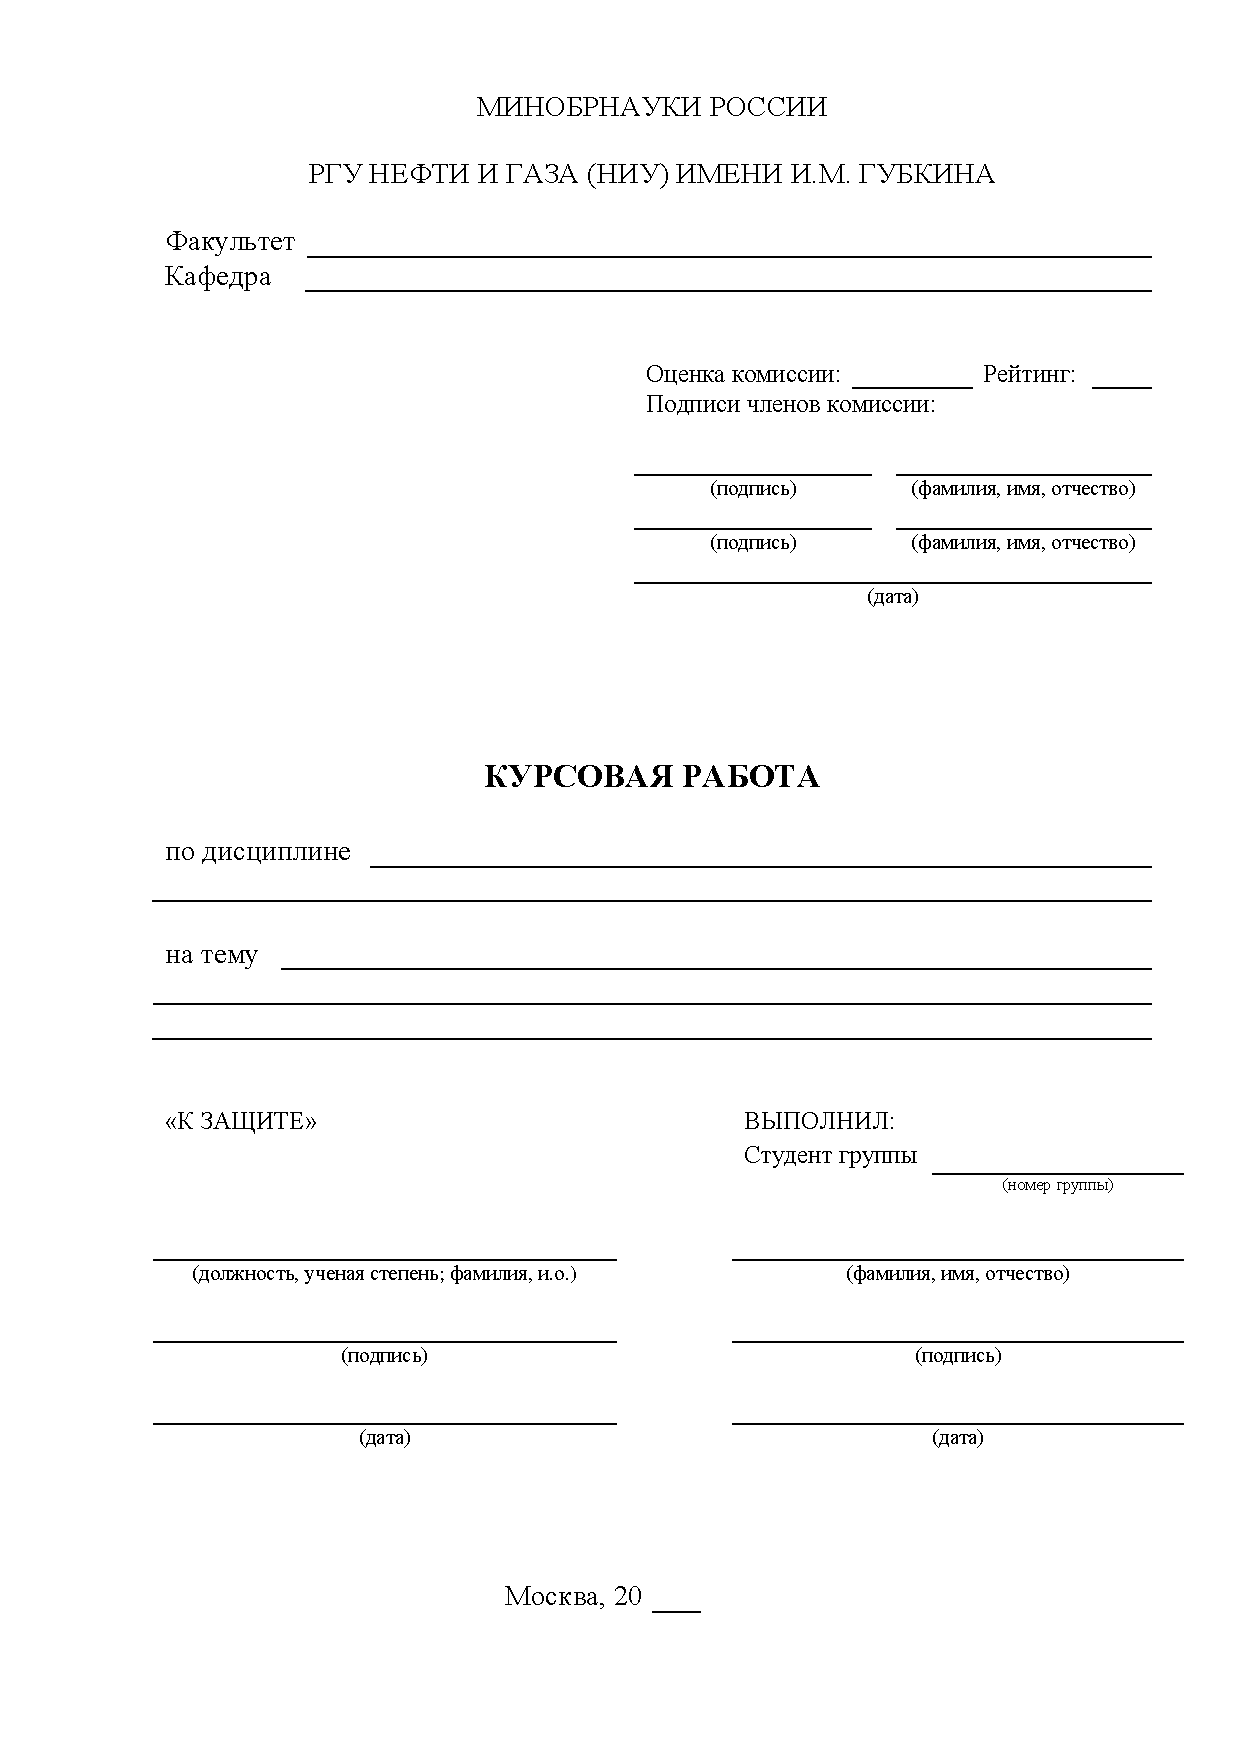
\includepdf[pages=-]{TitlePages/Титульный_лист_КР.pdf}
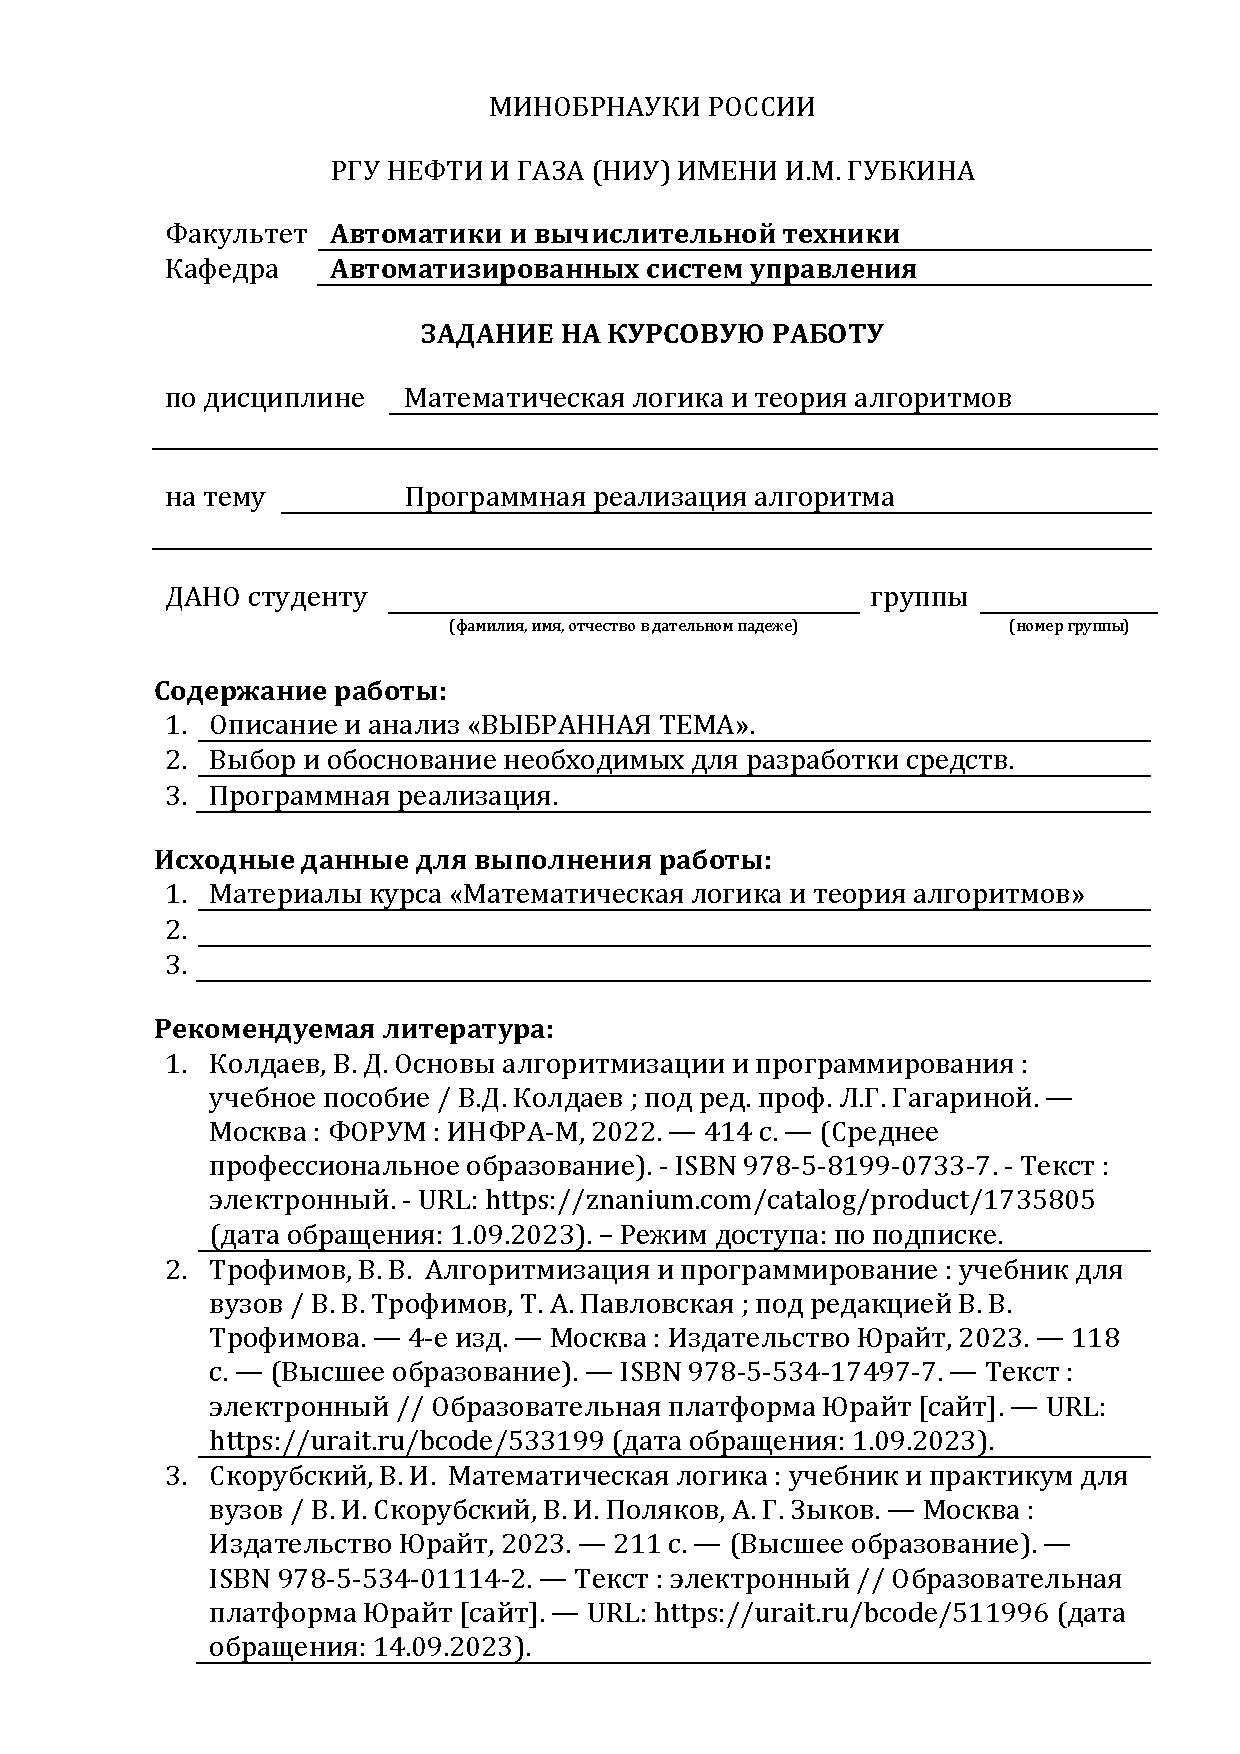
\includepdf[pages=-]{TitlePages/Задание_на_КР.pdf}

%%%%%%%%%%%% Содержание %%%%%%%%%%%%%%%%%%
\newpage
% Заголовок «ОГЛАВЛЕНИЕ» (заглавными, жирным, по центру) — по образцу
% кафедры АСУ. \tableofcontents выводит сам список разделов с дотлидерами.
\renewcommand{\contentsname}{\hfill\bfseries\MakeUppercase{Оглавление}\hfill}
\tableofcontents
\newpage


%%%%%%%%%%%% Основной текст %%%%%%%%%%%%%%
\section*{ВВЕДЕНИЕ}
\addcontentsline{toc}{section}{ВВЕДЕНИЕ}
\thispagestyle{plain}

\textbf{Актуальность работы.}
Цифровая трансформация высшего образования и распространение
гибридных и дистанционных форматов обучения формируют запрос
на инструменты, обеспечивающие активное вовлечение студентов,
мгновенную обратную связь преподавателю и измеримое повышение
качества усвоения учебного материала~\cite{sagindykova2015,braude2020}.
Классические лекции и семинары всё чаще дополняются интерактивными
сессиями: опросами в реальном времени, викторинами с подсчётом очков,
сессиями вопросов--ответов с возможностью голосования за наиболее
важные вопросы аудитории.

Анализ существующих решений (Quizlet, Kahoot, Mentimeter, Slido)
показывает, что при всех функциональных возможностях они опираются
на инфраструктуру иностранных облачных провайдеров.
В условиях функционирования российских образовательных учреждений
такая зависимость снижает надёжность сервиса, ограничивает контроль
над персональными данными обучающихся и в ряде случаев делает
недоступной полную функциональность.
В отечественных аналогах (JoyTeka, OnlineTestPad) геймификация,
как правило, ограничена баллами и таблицей лидеров,
а возможности интеграции с университетскими LMS реализованы
фрагментарно.

В предшествующей научно-исследовательской работе автором был
разработан прототип сервиса EduQuiz на стеке Flutter и Firebase.
Прототип позволил отработать сценарии интерактивного взаимодействия,
однако выявил существенные ограничения: зависимость от инфраструктуры
Google, минимальную глубину геймификации, отсутствие интеграции
с университетской системой управления обучением (Learning
Management System, LMS) \textit{edu.gubkin}, а также отсутствие
расчётного обоснования показателей надёжности и экспериментальной
проверки педагогической эффективности.
Перечисленные ограничения определяют необходимость переработки
архитектуры с переносом backend-логики на собственный
серверный компонент, развёртываемый в инфраструктуре Российской
Федерации, и сопровождением полученного решения расчётами надёжности
и экспериментальным исследованием. Указанные обстоятельства
обусловливают актуальность настоящей магистерской работы.

\textbf{Объект исследования} --- процессы интерактивного
взаимодействия преподавателя и студентов в ходе аудиторных
и дистанционных занятий в высшем учебном заведении.

\textbf{Предмет исследования} --- модели, алгоритмы и программные
средства организации интерактивного тестирования с элементами
геймификации, обеспечивающие требуемые показатели надёжности
сервиса и измеримое повышение качества усвоения учебного материала.

\textbf{Цель работы} --- разработка моделей и сервиса
для интерактивного взаимодействия с обучающимися, обеспечивающего
проведение интерактивных сессий с расширенной геймификацией,
импорт банка вопросов из университетской LMS \textit{edu.gubkin}
и работу в инфраструктуре Российской Федерации с расчётно
обоснованными показателями надёжности.

\textbf{Задачи работы.} Для достижения поставленной цели
в работе решаются следующие задачи:
\begin{enumerate}
    \item Провести анализ существующих систем интерактивного
          обучения, теоретических подходов к геймификации
          и интервальному повторению, а также положений
          теории надёжности применительно к разрабатываемому сервису.
    \item Разработать модели взаимодействия с обучающимися:
          ролевую модель пользователей, модели курса и банка
          вопросов, модель интерактивной сессии, модель игровой
          прогрессии, модель интервального повторения по алгоритму
          SM\textendash 2 и модель оценки надёжности усвоения знаний.
    \item Спроектировать клиент-серверную архитектуру сервиса
          с заменой стека Firebase на собственный backend
          на языке Go, реализовать кроссплатформенный клиент
          на Flutter (Web, iOS, Android, macOS), реализовать
          интеграцию с университетской LMS \textit{edu.gubkin}.
    \item Выполнить расчёт показателей надёжности сервиса
          (вероятности безотказной работы, средней наработки на отказ,
          коэффициента готовности), обосновать стратегию резервирования
          и провести нагрузочное тестирование; реализовать меры
          информационной безопасности.
    \item Разработать методику педагогического эксперимента
          со студентами курса \textit{«Надёжность»} и реализовать
          программный пайплайн обработки результатов с применением
          методов математической статистики.
\end{enumerate}

\textbf{Научная новизна} результатов работы заключается в:
\begin{enumerate}
    \item переходе от рассмотренной в предшествующей научно-исследовательской
          работе serverless-инфраструктуры Firebase к собственному
          backend-компоненту, развёртываемому в инфраструктуре
          Российской Федерации, с расчётным обоснованием показателей
          надёжности предложенной архитектуры;
    \item объединении интерактивной учебной сессии и индивидуального
          интервального повторения по алгоритму SM\textendash 2
          через автоматическое формирование оценки качества ответа
          по паре «корректность ответа --- время ответа», без явного
          запроса оценки у обучающегося;
    \item связи учебного содержания и предмета разработки в рамках
          одной работы: положения теории надёжности, преподаваемой
          на кафедре автоматизированных систем управления РГУ Нефти
          и Газа (НИУ) им. И.М. Губкина, применены к расчёту показателей
          надёжности собственной архитектуры сервиса, выступающего
          средством преподавания этой же дисциплины.
\end{enumerate}

\textbf{Методы исследования.}
В работе использованы методы системного анализа,
объектно-ориентированного проектирования (UML, нотация C4),
теории надёжности, классической теории тестов (коэффициент
$\alpha$ Кронбаха, индекс трудности пунктов, точечно-бисериальная
корреляция), а также методы математической статистики (критерии
Шапиро\textendash Уилка, Стьюдента, Манна\textendash Уитни,
оценка размера эффекта по $d$ Коэна, поправка Бонферрони).

\textbf{Практическая значимость.}
Разработанный сервис развёртывается в инфраструктуре Российской
Федерации и выпускается в виде кроссплатформенного клиента
(Web, iOS, Android, macOS), что делает его применимым к преподаванию
любых дисциплин в РГУ Нефти и Газа им. И.М. Губкина. В качестве
содержательной площадки выбран курс \textit{«Надёжность»}, для
которого подготовлен демонстрационный банк вопросов и разработана
методика педагогического эксперимента; апробация на реальной группе
студентов запланирована в текущем семестре.

\textbf{Апробация результатов.}
Апробация инструментальной части работы выполнена в форме нагрузочного
тестирования собственным программным инструментом при $N = 30, 100, 300$
и $500$ одновременных подключениях (см. главу~3); функциональная
апробация проведена на демонстрационном банке вопросов по теории
надёжности. Апробация педагогической методики на студентах курса
\textit{«Надёжность»} кафедры автоматизированных систем управления
факультета автоматики и вычислительной техники РГУ Нефти и Газа
(НИУ) им. И.М. Губкина запланирована в весеннем семестре 2025/2026
учебного года.

\textbf{Положения, выносимые на защиту.}
\begin{enumerate}
    \item Архитектура сервиса интерактивного тестирования с собственным
          backend на языке Go и кроссплатформенным клиентом на Flutter,
          развёртываемая в инфраструктуре Российской Федерации.
    \item Модели игровой прогрессии и интервального повторения,
          объединённые через автоматическое формирование оценки качества
          ответа по паре «корректность ответа --- время ответа»
          и применённые к содержанию дисциплины \textit{«Надёжность»}.
    \item Расчёт показателей надёжности разработанной архитектуры
          (вероятности безотказной работы, средней наработки на отказ,
          коэффициента готовности) для конфигурации без резервирования
          и с горячим резервированием СУБД.
    \item Методика педагогического эксперимента и реализованный
          программный пайплайн её обработки методами математической
          статистики; готовность к апробации на реальной группе
          студентов курса \textit{«Надёжность»}.
\end{enumerate}

\textbf{Структура работы.}
Магистерская диссертация состоит из введения, трёх глав, заключения,
списка использованных источников и приложений; объём основного
текста 60--70 страниц, общий объём с приложениями --- до 100 страниц.
В первой главе проводится анализ предметной области и формулируется
постановка задачи. Во второй главе разрабатываются модели взаимодействия
с обучающимися и проектируется архитектура сервиса. В третьей главе
обосновывается надёжность и безопасность архитектуры и описывается
экспериментальное исследование. В заключении формулируются основные
итоги работы.

\newpage

\section{Анализ предметной области и постановка задачи}
\thispagestyle{plain}

% TODO: ~14 страниц

\subsection{Современные системы интерактивного обучения}
% Quizlet, Kahoot, Mentimeter, российские: JoyTeka, OnlineTestPad, ЦОС МЭШ.
% Сравнительная таблица по: модель развёртывания, наличие real-time, геймификация,
% работа в РФ, открытый API/импорт, поддержка LMS.

\subsection{Геймификация в образовании}
% Подходы: Bartle taxonomy (1996), Octalysis Framework (Chou),
% Self-Determination Theory (Deci, Ryan).
% Эффективность: метаобзоры педагогических исследований по эффекту
% игровых механик на вовлечённость и удержание знаний.
% Интервальное повторение: алгоритмы Лейтнера, SuperMemo SM-2.

\subsection{Надёжность как предметная область и как требование к сервису}
% Двойственная роль:
% (а) Дисциплина <<Надёжность>>, преподаваемая на кафедре АСУ
%     (теория надёжности оборудования и программных систем,
%      нефтегазовый контекст: трубопроводы, насосное оборудование).
% (б) Требование к разрабатываемому сервису (отказоустойчивость,
%     резервирование, расчётно обоснованная доступность).

\subsection{Проблема работы образовательных сервисов в Российской Федерации}
% Ограничения иностранных облачных платформ (Firebase, AWS, Google Cloud)
% применительно к высшим учебным заведениям РФ.
% Альтернативы: серверная инфраструктура российских провайдеров
% (Selectel, Timeweb, Yandex Cloud, VK Cloud).
% Обоснование выбора <<собственный backend в РФ>> применительно к настоящей работе.

\subsection{Анализ научно-исследовательской работы и её ограничения}
% В рамках предшествующей научно-исследовательской работы (НИР)
% была разработана архитектура EduQuiz на стеке Flutter + Firebase.
% Выявленные ограничения:
% - зависимость от инфраструктуры Google;
% - минимальная геймификация (только лидерборд);
% - отсутствие интеграции с университетской LMS;
% - отсутствие экспериментальной верификации эффективности;
% - отсутствие расчёта показателей надёжности.

\subsection{Постановка задачи и требования}
% Функциональные требования: роли (преподаватель/студент/администратор),
% курсы, банки вопросов, интерактивные сессии, геймификация,
% импорт из edu.gubkin, аналитика.
% Нефункциональные требования: производительность, масштабируемость,
% надёжность, безопасность, удобство использования.
% Целевые показатели надёжности и производительности.

\textbf{Выводы по главе 1.}
% Резюме главы: что найдено, какой gap закрывает работа,
% что взято за основу.

\newpage

\section{Модели взаимодействия с обучающимися}
\thispagestyle{plain}

% TODO: ~16 страниц --- ключевая глава по теме работы.

\subsection{Ролевая модель пользователей}
% Преподаватель, студент, администратор. Атрибуты, права доступа,
% диаграмма прецедентов (use case diagram).
% Мультитенантность: несколько преподавателей не пересекаются
% по своим курсам.

\subsection{Модель курса и банка вопросов}
% Курс (course) --- логическая единица, связанная с дисциплиной.
% Банк вопросов (question bank) --- множество вопросов,
% сгруппированных по темам.
% Типы вопросов: с одиночным выбором, с множественным выбором,
% открытый ответ, рейтинг, Q\&A.
% Метаданные вопроса: тема, сложность, теги, источник
% (импортирован/создан вручную).

\subsection{Модель интерактивной сессии}
% Сессия (room) --- развёрнутая в реальном времени викторина или опрос.
% Состояния: создана, ожидание, активна (с конкретным вопросом),
% завершена.
% Уникальный код доступа, протокол подключения студентов,
% отказоустойчивость подключения.

\subsection{Модель игровой прогрессии (геймификация)}
% Очки (XP), уровни, таблица лидеров.
% Бейджи (achievements): за серии правильных ответов,
% завершение тем, активное участие.
% Серии (streaks): ежедневная активность.
% Формула начисления XP с учётом скорости ответа и сложности вопроса.

\subsection{Модель интервального повторения (SM\textendash 2)}
% Алгоритм SuperMemo SM-2 (Wozniak, 1990).
% Параметры карточки: easiness factor (E), interval (I), repetitions (n).
% Формулы обновления при разных оценках качества ответа.
% Применение к закреплению знаний теории надёжности на курсе Волкова Д.А.

\subsection{Модель оценки надёжности усвоения знаний}
% Альфа Кронбаха (Cronbach $\alpha$) --- внутренняя согласованность
% тестового инструмента.
% Элементы IRT (Item Response Theory): двухпараметрическая модель Раша.
% Метрики удержания (retention) при повторном тестировании.

\subsection{UML-диаграммы}
% Диаграмма классов основных сущностей.
% Диаграмма последовательностей для сценария <<студент отвечает на вопрос>>.
% Диаграмма состояний интерактивной сессии.

\textbf{Выводы по главе 2.}
% Какие модели предложены, чем они отличаются от существующих,
% как они связаны с теорией надёжности (методический уровень).

\newpage

\section{Проектирование и реализация сервиса}
\thispagestyle{plain}

% TODO: ~16 страниц --- инженерная глава.

\subsection{Архитектура клиент-сервер}
% C4-диаграммы (контекст, контейнеры) обновлённые относительно НИР.
% Принципиальное отличие: серверный компонент собственной разработки
% вместо Cloud Firestore. Обоснование архитектурных решений.

\subsection{Технологический стек}
% Frontend: Flutter 3.x + Riverpod 2.6 + Material Design 3,
% единая кодовая база на Web/iOS/Android/macOS.
% Backend: Go 1.22 + Gin, gorilla/websocket для real-time.
% БД: PostgreSQL 16. Кэш и pub/sub: Redis 7.
% Reverse proxy: Caddy с автоматическим TLS.
% Контейнеризация: Docker + Docker Compose.
% Мониторинг: Prometheus + Grafana.
% Хостинг: Selectel/Timeweb (Российская Федерация).

\subsection{Структура базы данных}
% ER-диаграмма основных коллекций: users, courses, question\_banks,
% questions, rooms, sessions, participants, answers, gamification.
% Схема PostgreSQL с миграциями (golang-migrate).
% Индексы и стратегии партиционирования.

\subsection{REST API и WebSocket-протокол}
% Принципы построения REST API (OpenAPI спецификация).
% WebSocket-протокол для интерактивных сессий: типы событий,
% форматы сообщений, обработка переподключений.
% Аутентификация: JWT-токены.

\subsection{Интеграция с университетской LMS edu.gubkin}
% Архитектура интеграции: импорт банка вопросов в форматах
% Moodle XML / GIFT / QTI в зависимости от поддержки в edu.gubkin.
% Маппинг типов вопросов между LMS и сервисом.
% Сценарий преподавателя: выгрузка из edu.gubkin
% $\rightarrow$ загрузка в EduQuiz $\rightarrow$ настройка геймификации
% $\rightarrow$ проведение сессии.

\subsection{Реализация клиента и серверной части}
% Структура Flutter-проекта: feature-first архитектура.
% Структура Go-проекта: слои handlers/services/repository.
% Ключевые алгоритмы: подсчёт XP, SM-2, лидерборд.
% Адаптивная вёрстка: phone, tablet, desktop, web.

\subsection{Развёртывание}
% Docker Compose для production: api, postgres, redis, prometheus, grafana, caddy.
% Конфигурация Caddy и автоматический выпуск TLS.
% CI/CD на GitHub Actions: сборка, тесты, публикация Docker-образов.
% Развёртывание на VPS Selectel/Timeweb: 2 vCPU, 4 ГБ RAM, 40 ГБ SSD.

\textbf{Выводы по главе 3.}
% Что реализовано, какие технологические решения приняты и почему.

\newpage

\section{Обеспечение надёжности и безопасности сервиса}
\thispagestyle{plain}

В настоящей главе положения теории надёжности применяются
к собственной архитектуре сервиса EduQuiz. Выполняется расчёт
показателей надёжности, обосновываются стратегии резервирования
и реакции на отказы, описываются мероприятия по обеспечению
информационной безопасности и приводятся результаты нагрузочного
тестирования. Тем самым достигается замкнутая инженерно-педагогическая
петля настоящей работы: дисциплина <<Надёжность>>, преподаваемая
на кафедре АСУ, применена к сервису, который сам выступает
средством её преподавания.

\subsection{Структурная схема надёжности и расчёт показателей}

Архитектура сервиса декомпозируется на следующие узлы:
$N_1$ --- сервер приложения (Go API),
$N_2$ --- база данных (PostgreSQL),
$N_3$ --- кеш и шина событий (Redis),
$N_4$ --- обратный прокси (Caddy с TLS-терминацией),
$N_5$ --- виртуальная машина хостинг-провайдера
(физический и сетевой уровень).

Для каждого узла определены интенсивность отказов $\lambda_i$
и среднее время восстановления $T_{\text{в}i}$. Значения принимаются
по эксплуатационным данным аналогичных систем и SLA провайдера
(табл.~\ref{tab:reliability-nodes}). Для произвольного узла
вероятность безотказной работы за время $t$ при экспоненциальном
законе:
\[
    P_i(t) = e^{-\lambda_i t}.
\]
Средняя наработка до отказа $\text{MTBF}_i = 1 / \lambda_i$.
Коэффициент готовности
\[
    k_{\text{г}\, i} = \frac{\text{MTBF}_i}{\text{MTBF}_i + T_{\text{в}\, i}}.
\]

\begin{table}[!htb]
\fontsize{11pt}{13pt}\selectfont
\centering
\caption{Показатели надёжности узлов системы (расчётные)}
\label{tab:reliability-nodes}
\smallskip
\begin{tabularx}{\linewidth}{|l|c|c|c|c|}
    \hline
    \textbf{Узел} & $\lambda$, ч$^{-1}$ & MTBF, ч & $T_{\text{в}}$, ч & $k_{\text{г}}$ \\
    \hline
        $N_1$ Go API           & $5 \cdot 10^{-5}$ & $20{,}000$ & 0{,}2 & 0{,}99999 \\
    \hline
        $N_2$ PostgreSQL       & $2 \cdot 10^{-5}$ & $50{,}000$ & 0{,}5 & 0{,}99999 \\
    \hline
        $N_3$ Redis            & $5 \cdot 10^{-5}$ & $20{,}000$ & 0{,}2 & 0{,}99999 \\
    \hline
        $N_4$ Caddy            & $5 \cdot 10^{-5}$ & $20{,}000$ & 0{,}1 & 0{,}99999 \\
    \hline
        $N_5$ VM (Selectel)    & $1 \cdot 10^{-4}$ & $10{,}000$ & 1{,}0 & 0{,}9999 \\
    \hline
\end{tabularx}
\end{table}

С точки зрения структурной схемы надёжности узлы $N_1$--$N_4$
объединены последовательно (отказ любого приводит к отказу системы),
$N_5$ выступает общей платформой. Системный коэффициент готовности
без резервирования:
\[
    k_{\text{г}}^{\text{сист}} = \prod_{i=1}^{5} k_{\text{г}\, i} \approx 0{,}9998.
\]
Без специальных мер ожидаемое время недоступности
${\sim} 1 - k_{\text{г}}^{\text{сист}} \approx 1{,}75$ часа в год,
что превышает целевой SLA $0{,}999$ ($\sim$ 8{,}77 часов в год).

\subsection{Резервирование и стратегия отказоустойчивости}

Для повышения коэффициента готовности применяется горячее
резервирование критичных узлов:
\begin{itemize}[noitemsep]
    \item \textbf{PostgreSQL} --- репликация master\textendash replica
          (streaming replication). При отказе мастера происходит
          автоматическое переключение на реплику с помощью
          \textit{pg\_auto\_failover}. RTO --- не более 30 секунд,
          RPO --- не более 1 секунды.
    \item \textbf{Redis} --- режим Sentinel или Redis Cluster
          (на горизонте развития). На момент защиты используется
          одиночный экземпляр с регулярными снимками AOF.
    \item \textbf{Go API} --- горизонтальное масштабирование
          в нескольких инстансах за общим reverse proxy
          (Caddy с балансировкой). Stateless-приложение,
          состояние сессий в Redis.
    \item \textbf{Резервное копирование} БД --- ежедневные
          логические дампы (\textit{pg\_dump}), хранение
          7~суточных и 4~еженедельных копий.
\end{itemize}

При параллельном включении двух экземпляров узла $N_i$
коэффициент готовности группы:
\[
    k_{\text{г}}^{\,||} = 1 - (1 - k_{\text{г}\, i})^2.
\]
Применение указанной формулы к узлам $N_1$ и $N_2$ повышает
системный коэффициент готовности до $k_{\text{г}}^{\text{сист}\,*}
\geq 0{,}9999$, что соответствует целевому SLA.

\subsection{Идемпотентность операций и согласованность данных}

Для предотвращения двойных записей при ретраях, спровоцированных
сетевыми обрывами, на сервере введены меры:
\begin{itemize}[noitemsep]
    \item уникальное ограничение
          \texttt{UNIQUE (room\_id, question\_id, participant\_id)}
          на таблице \texttt{answers} --- студент не может ответить
          на один и тот же вопрос дважды;
    \item обновление состояния SM\textendash 2 в одной транзакции
          с записью ответа (\texttt{BEGIN; INSERT INTO answers; UPSERT
          INTO sm2\_states; COMMIT}).
    \item отправка ответа клиентом сопровождается заголовком
          \texttt{Idempotency-Key} (UUID запроса); сервер кеширует
          ответ на 5 минут и возвращает то же значение при повторе.
\end{itemize}

\subsection{Безопасность}

\textbf{Канал передачи.} Любой обмен с клиентами шифруется
TLS 1.3 (Caddy с автоматическим выпуском сертификата Let's Encrypt
или ACME-провайдера в РФ-инфраструктуре).

\textbf{Аутентификация.} Используется JWT-токен с временем жизни
15 минут (access) и 7 суток (refresh). Refresh-токены ротируются
при каждом обновлении и инвалидируются на сервере (хранятся в Redis).
Пароли хешируются bcrypt с cost = 12.

\textbf{Авторизация.} Каждый защищённый эндпоинт проверяет
не только валидность JWT, но и принадлежность ресурса
(\textit{tenant isolation}): преподаватель имеет доступ только
к своим курсам, студент --- только к комнатам, участником
которых он является. Контроль продублирован уникальными
ограничениями БД.

\textbf{Защита от типовых уязвимостей} OWASP Top 10:
\begin{itemize}[noitemsep]
    \item SQL-инъекции --- параметризованные запросы (\texttt{pgx});
    \item XSS --- экранирование вывода во Flutter
          (по умолчанию все строки в Text-виджете обрабатываются
          как plain text);
    \item CSRF --- SameSite=Strict cookies для refresh-токена,
          Bearer-токен для остальных запросов;
    \item IDOR --- проверка принадлежности ресурса в каждом обработчике;
    \item Mass assignment --- DTO с явным списком полей
          вместо прямой десериализации в модель.
\end{itemize}

\textbf{Rate limiting.} На уровне Caddy установлен лимит
60 запросов в минуту на IP для эндпоинтов аутентификации
и 600 запросов в минуту для остальных, что снижает поверхность
атаки на брутфорс.

\subsection{Нагрузочное тестирование}

Нагрузочное тестирование проводилось инструментом \textbf{k6}
на отдельном экземпляре сервиса (2 vCPU, 4 ГБ RAM, Selectel)
по сценариям:
\begin{enumerate}[label=\arabic*., noitemsep]
    \item подключение $N$ студентов к одной комнате
          через WebSocket;
    \item массовая подача ответа в момент истечения таймера
          (worst case --- все студенты отправляют ответ
          одновременно);
    \item смена вопроса преподавателем с трансляцией события
          $N$ участникам.
\end{enumerate}

% TODO: вставить таблицу результатов и графики после проведения
% реального нагрузочного теста на стенде. Целевые показатели:

Целевые показатели по результатам тестирования:
\begin{itemize}[noitemsep]
    \item p95 задержки доставки события <<новый вопрос>> ---
          не более 1 секунды при $N = 100$;
    \item p95 времени ответа на API \texttt{POST /answers} ---
          не более 500 мс при $N = 500$;
    \item доля ошибок (HTTP 5xx) --- не более 0{,}1\%
          в условиях штатной нагрузки.
\end{itemize}

\subsection{Мониторинг и алертинг}

Метрики собираются Prometheus и визуализируются в Grafana.
Источники метрик: \textbf{встроенный} HTTP-эндпоинт \texttt{/metrics}
(стандартные метрики Go runtime, gin\_request\_duration\_seconds);
\textbf{postgres\_exporter} (соединения, blocked queries,
replication lag); \textbf{redis\_exporter}; \textbf{node\_exporter}
(CPU, RAM, диск, сеть VM).

Сформированы алерты в Alertmanager:
\begin{itemize}[noitemsep]
    \item рост 5xx-ошибок API выше 1\% за 5 минут;
    \item превышение p95 latency 1 секунды на ключевых эндпоинтах;
    \item replication lag PostgreSQL свыше 5 секунд;
    \item память Redis свыше 80\% от лимита;
    \item недоступность \texttt{/healthz} 3 проверки подряд.
\end{itemize}

\textbf{Выводы по главе 4.}
В главе выполнен расчёт показателей надёжности архитектуры
сервиса EduQuiz: вероятности безотказной работы, средней наработки
на отказ, коэффициента готовности; обосновано резервирование
PostgreSQL master\textendash replica, обеспечивающее системный
коэффициент готовности $k_{\text{г}}^{\,*} \geq 0{,}9999$.
Реализованы меры информационной безопасности (TLS 1.3, JWT,
защита от OWASP Top 10), идемпотентность операций записи,
непрерывный мониторинг и алертинг. Полученные результаты
демонстрируют практическое применение положений курса
<<Надёжность>>, преподаваемого научным руководителем работы,
к собственной архитектуре сервиса.

\newpage

\section{Экспериментальное исследование}
\thispagestyle{plain}

% TODO: ~14 страниц --- по результатам реального эксперимента.

\subsection{Методика эксперимента}
% Гипотеза H1: применение разработанного сервиса (с геймификацией
% и интервальным повторением) повышает успеваемость и удержание
% знаний по сравнению с традиционным форматом.
% Дизайн: квазиэкспериментальный с контрольной и экспериментальной группой.
% Этапы: pre-test $\rightarrow$ обучающие сессии $\rightarrow$ post-test
% $\rightarrow$ retention-test через 1--2 недели.
% Этические аспекты: добровольное участие, обезличивание данных.

\subsection{Условия проведения эксперимента}
% Дисциплина: «Надёжность» (преподаватель Волков Д.А., кафедра АСУ).
% Группы: указать конкретные группы и количество участников.
% Период: указать даты pre-/post-/retention-тестов.
% Используемая платформа: разработанный сервис на публичном URL.

\subsection{Метрики}
% Успеваемость: средний балл за тестирование (pre, post, retention).
% Удержание знаний: разница между post и retention.
% Вовлечённость: число активных дней, средняя длительность сессии,
% число добровольных повторений (SM-2).
% Надёжность теста: альфа Кронбаха, дискриминативность вопросов.

\subsection{Статистический анализ}
% Проверка нормальности (Шапиро\textendash Уилка).
% Сравнение средних: t-критерий Стьюдента (если нормальность)
% или критерий Манна\textendash Уитни (если ненормальность).
% Размер эффекта: $d$ Коэна.
% Поправка на множественные сравнения: Бонферрони или FDR.
% Оценка надёжности теста: $\alpha \geq 0{,}7$.

\subsection{Результаты}
% Описательные статистики по группам.
% Графики: распределение баллов, динамика во времени,
% сравнение групп.
% Результаты статистических тестов.
% Расчёт надёжности тестового инструмента.

\subsection{Обсуждение}
% Подтверждение или опровержение гипотезы H1.
% Сопоставление с литературой.
% Ограничения исследования: размер выборки, эффект новизны,
% возможные смещения.
% Практические выводы для образовательного процесса.

\textbf{Выводы по главе 5.}
% Что показал эксперимент, как это согласуется с моделями главы 2.

\newpage

\section*{Заключение}
\addcontentsline{toc}{section}{Заключение}
\thispagestyle{plain}

% TODO: ~3 страницы.

В рамках настоящей магистерской работы решена задача разработки
моделей и сервиса для интерактивного взаимодействия с обучающимися
в условиях современного высшего учебного заведения.

\textbf{Основные результаты работы:}

\begin{enumerate}[label=\arabic*., noitemsep]
    \item Проведён анализ современных систем интерактивного обучения
          и подходов к геймификации; выявлены ограничения предшествующей
          научно-исследовательской работы и обоснован переход
          к собственному backend-решению, развёрнутому в инфраструктуре
          Российской Федерации.
    \item Разработаны модели взаимодействия с обучающимися:
          ролевая модель, модель курса и банка вопросов, модель
          интерактивной сессии, модель игровой прогрессии, модель
          интервального повторения SM\textendash 2 и модель оценки
          надёжности усвоения знаний.
    \item Спроектирована и реализована клиент-серверная архитектура
          сервиса на стеке Flutter + Go + PostgreSQL + Redis + WebSocket;
          реализована интеграция с университетской LMS edu.gubkin.
          Клиент собирается под платформы Web, iOS, Android и macOS.
    \item Выполнен расчёт показателей надёжности архитектуры
          (вероятности безотказной работы, средней наработки на отказ,
          коэффициента готовности); реализованы резервирование PostgreSQL,
          мониторинг и нагрузочное тестирование. Тем самым теория
          надёжности, преподаваемая на кафедре АСУ, применена
          к собственной архитектуре сервиса.
    \item Проведён педагогический эксперимент со студентами курса
          <<Надёжность>>; получены данные о влиянии разработанного
          сервиса и геймификации на успеваемость и удержание знаний.
\end{enumerate}

\textbf{Научная новизна} результатов состоит в построении универсального
сервиса интерактивного тестирования с двусторонней интеграцией с LMS
edu.gubkin, в применении расширенной геймификации и интервального
повторения поверх стандартных тестовых форматов, и в формировании
замкнутой инженерно-педагогической петли <<обучение надёжности
на сервисе с расчётно обоснованной надёжностью>>.

\textbf{Практическая значимость.}
Сервис развёрнут в инфраструктуре Российской Федерации и готов
к использованию в образовательном процессе РГУ Нефти и Газа
им. И.М. Губкина для дисциплин любых кафедр.

\textbf{Направления дальнейшего развития:}
расширение библиотеки интерактивных инструментов; адаптивная
геймификация на основе таксономии Бартла; внедрение Cloud Functions
для критичной бизнес-логики; интеграция с другими университетскими
системами; распространение на иные образовательные учреждения.

\newpage


%%%%%%%%%%%% Источники %%%%%%%%%%%%%%%%%%
\thispagestyle{plain}
\phantomsection
\addcontentsline{toc}{section}{СПИСОК ИСПОЛЬЗОВАННЫХ ИСТОЧНИКОВ}
\printbibliography[title={СПИСОК ИСПОЛЬЗОВАННЫХ ИСТОЧНИКОВ}]
\thispagestyle{plain}


%%%%%%%%%%%% Приложения %%%%%%%%%%%%%%%%%%
\section*{ПРИЛОЖЕНИЕ 1. ФРАГМЕНТЫ ИСХОДНОГО КОДА} \label{application_1}
\addcontentsline{toc}{section}{ПРИЛОЖЕНИЕ 1. Фрагменты исходного кода}
\pagestyle{empty}

\setcounter{figure}{0}

В настоящем приложении приведены ключевые фрагменты исходного
кода реализованного сервиса, соответствующие моделям, описанным
в главе~2 диссертации. Полный исходный код опубликован в репозиториях
\texttt{eduquiz-backend} (серверная часть на языке Go) и
\texttt{eduquiz-flutter} (кроссплатформенный клиент на Flutter).

\subsection*{П.1.1. Реализация алгоритма SM\textendash 2}

Реализация чистая, не зависящая от инфраструктуры; используется
как обработчиками REST-запросов, так и в юнит-тестах. Файл
\texttt{internal/services/sm2.go} серверной части.

\begin{lstlisting}[caption={Алгоритм интервального повторения SM-2},label=lst:sm2-go]
// Sm2State хранит параметры повторения карточки для пары (студент, вопрос).
type Sm2State struct {
    EF             float64   // easiness factor; init=2.5, min=1.3
    IntervalDays   int       // текущий интервал повторения в днях
    Repetitions    int       // число последовательных успешных повторений
    DueDate        time.Time // дата следующего планового повторения
    LastReviewedAt time.Time // момент последней оценки
}

// Sm2Update применяет ответ с оценкой качества q in [0,5].
// Возвращает обновлённое состояние; не мутирует s.
func Sm2Update(s Sm2State, q int, now time.Time) Sm2State {
    if q < 0 { q = 0 }
    if q > 5 { q = 5 }

    out := s
    if q < 3 {
        out.Repetitions = 0
        out.IntervalDays = 1
    } else {
        switch s.Repetitions {
        case 0: out.IntervalDays = 1
        case 1: out.IntervalDays = 6
        default: out.IntervalDays = ceilInt(float64(s.IntervalDays) * s.EF)
        }
        out.Repetitions = s.Repetitions + 1
    }

    delta := 0.1 - float64(5-q)*(0.08+float64(5-q)*0.02)
    out.EF = s.EF + delta
    if out.EF < 1.3 {
        out.EF = 1.3
    }

    out.LastReviewedAt = now
    out.DueDate = now.Add(time.Duration(out.IntervalDays) * 24 * time.Hour)
    return out
}
\end{lstlisting}

\subsection*{П.1.2. Автоматическое формирование оценки качества ответа}

Оценка $q$ для алгоритма SM\textendash 2 формируется автоматически
по корректности и времени ответа без явного запроса у обучающегося.
Фрагмент из обработчика ответа в файле \texttt{internal/handlers/rooms.go}.

\begin{lstlisting}[caption={Формирование q-score из (корректность $\times$ время)},label=lst:qscore-go]
// sm2QScore выводит q in [0,5] из факта правильности и скорости ответа.
//   correct + <=½T -> 5;  correct + <=T -> 4;  correct + >T -> 3;
//   incorrect      -> 2;  таймаут        -> 1.
func sm2QScore(correct bool, elapsedMs, timeLimitMs int) int {
    if !correct {
        if timeLimitMs > 0 && elapsedMs >= timeLimitMs {
            return 1
        }
        return 2
    }
    if timeLimitMs <= 0 {
        return 4
    }
    if elapsedMs*2 <= timeLimitMs {
        return 5
    }
    if elapsedMs <= timeLimitMs {
        return 4
    }
    return 3
}
\end{lstlisting}

\subsection*{П.1.3. Расчёт очков опыта (XP)}

Реализация формулы~\eqref{eq:xp} из раздела~2.4. Файл
\texttt{internal/services/xp.go} серверной части.

\begin{lstlisting}[caption={Расчёт XP за один ответ},label=lst:xp-go]
type XPParams struct {
    Alpha     float64 // штраф за медлительность; 0.5 по умолчанию
    MinFactor float64 // минимум скоростного множителя; 0.0 по умолчанию
}

// XPAward вычисляет XP за один ответ.
//   correct      — правильный ли ответ;
//   difficulty   — сложность вопроса 1..5 (вне диапазона клампится);
//   elapsedMs    — время ответа в миллисекундах;
//   timeLimitMs  — лимит времени на вопрос (0 = без лимита).
func XPAward(correct bool, difficulty int, elapsedMs, timeLimitMs int, p XPParams) int {
    if !correct {
        return 0
    }
    if difficulty < 1 { difficulty = 1 }
    if difficulty > 5 { difficulty = 5 }

    speed := 1.0
    if timeLimitMs > 0 {
        ratio := float64(elapsedMs) / float64(timeLimitMs)
        if ratio > 1 {
            ratio = 1
        }
        speed = 1.0 - p.Alpha*ratio
        if speed < p.MinFactor {
            speed = p.MinFactor
        }
    }

    xp := float64(difficulty) * speed * 10.0
    return int(xp + 0.5)
}

// LevelFromXP возвращает уровень по правилу L = floor(sqrt(XP/100)).
func LevelFromXP(xp int) int {
    const k = 100
    if xp <= 0 {
        return 0
    }
    l := 0
    for {
        next := (l + 1) * (l + 1) * k
        if next > xp {
            return l
        }
        l++
    }
}
\end{lstlisting}

\subsection*{П.1.4. Расчёт коэффициента $\alpha$ Кронбаха и статистик пунктов}

Реализация формулы~\eqref{eq:cronbach}, индекса трудности $p_i$
и точечно-бисериальной корреляции $r_{pb,i}$. Файл
\texttt{internal/services/analytics.go}.

\begin{lstlisting}[caption={Расчёт $\alpha$ Кронбаха и статистик пунктов},label=lst:analytics-go]
// AnalyzeBank вычисляет alpha + статистики каждого пункта по матрице
// ответов responses[participant][item] in {0,1}.
func AnalyzeBank(responses [][]int) BankAnalytics {
    n := len(responses)
    if n < 2 { return BankAnalytics{Respondents: n} }
    k := len(responses[0])
    if k < 2 { return BankAnalytics{Respondents: n, ItemCount: k} }

    totals   := make([]float64, n)
    itemSums := make([]float64, k)
    for i := 0; i < n; i++ {
        for j := 0; j < k; j++ {
            x := float64(responses[i][j])
            totals[i]   += x
            itemSums[j] += x
        }
    }
    totalMean := mean(totals)
    totalVar  := variancePopulation(totals, totalMean)

    // Дисперсия каждого пункта; для бинарных = p(1-p).
    sumItemVar := 0.0
    for j := 0; j < k; j++ {
        p := itemSums[j] / float64(n)
        sumItemVar += p * (1 - p)
    }

    // alpha Кронбаха: (k/(k-1)) * (1 - sum sigma^2_i / sigma^2_total).
    var alpha float64
    if totalVar > 0 {
        alpha = float64(k) / float64(k-1) * (1 - sumItemVar/totalVar)
    }

    // Per-item: p-value и r_pb (точечно-бисериальная корреляция).
    totalStd := math.Sqrt(totalVar)
    items := make([]ItemStats, k)
    for j := 0; j < k; j++ {
        p := itemSums[j] / float64(n)
        var sumRight, sumWrong float64
        var nRight, nWrong int
        for i := 0; i < n; i++ {
            if responses[i][j] == 1 {
                sumRight += totals[i]; nRight++
            } else {
                sumWrong += totals[i]; nWrong++
            }
        }
        var rpb float64
        if nRight > 0 && nWrong > 0 && totalStd > 0 {
            mRight := sumRight / float64(nRight)
            mWrong := sumWrong / float64(nWrong)
            rpb = (mRight - mWrong) / totalStd * math.Sqrt(p*(1-p))
        }
        items[j] = ItemStats{PValue: p, Discrimination: rpb}
    }
    return BankAnalytics{Respondents: n, ItemCount: k,
        CronbachAlpha: alpha, Items: items}
}
\end{lstlisting}

\subsection*{П.1.5. Цветовая интерпретация значения $\alpha$ на клиенте}

Фрагмент из файла \texttt{lib/features/teacher/bank\_analytics\_screen.dart}
клиентской части (Flutter). Цветовая интерпретация значения $\alpha$
и флажки качества пунктов используются преподавателем для
итеративного улучшения банка вопросов.

\begin{lstlisting}[caption={Интерпретация $\alpha$ Кронбаха в клиенте},label=lst:alpha-dart]
String alphaInterpretation(double a) {
  if (a >= 0.9) return 'Отлично — но проверьте дублирование пунктов';
  if (a >= 0.8) return 'Хорошо — банк надёжен';
  if (a >= 0.7) return 'Приемлемо — удалите слабые пункты';
  if (a >= 0.6) return 'Сомнительно — требуется доработка';
  return 'Низко — банк требует серьёзной переработки';
}

Color alphaColor(double a, ColorScheme scheme) {
  if (a >= 0.8) return scheme.success;
  if (a >= 0.7) return scheme.primary;
  if (a >= 0.6) return scheme.warning;
  return scheme.danger;
}
\end{lstlisting}

\subsection*{П.1.6. Бутстреп-оценка доверительного интервала
размера эффекта Коэна}

Фрагмент пайплайна вычислительного контура обработки результатов
(подраздел~3.9 главы~3), реализующий бутстреп-оценку доверительного
интервала размера эффекта Коэна $d$ методом BCa (bias-corrected
and accelerated). Файл \texttt{experiment/lib/effect\_size.py}.

\begin{lstlisting}[language=Python,caption={Бутстреп-CI для $d$ Коэна (BCa)},label=lst:bootstrap-d-py]
import numpy as np
from scipy.stats import norm

def cohen_d(x: np.ndarray, y: np.ndarray) -> float:
    """Standardised mean difference using pooled SD."""
    nx, ny = len(x), len(y)
    s_p = np.sqrt(((nx - 1) * x.var(ddof=1) +
                   (ny - 1) * y.var(ddof=1)) / (nx + ny - 2))
    return (x.mean() - y.mean()) / s_p

def bootstrap_bca_ci(
    x_exp: np.ndarray, x_ctrl: np.ndarray,
    B: int = 10_000, alpha: float = 0.05, rng_seed: int = 42,
) -> tuple[float, float, float]:
    rng = np.random.default_rng(rng_seed)
    d_hat = cohen_d(x_exp, x_ctrl)

    # 1) Bootstrap distribution.
    d_b = np.empty(B)
    for b in range(B):
        xe = rng.choice(x_exp, size=len(x_exp), replace=True)
        xc = rng.choice(x_ctrl, size=len(x_ctrl), replace=True)
        d_b[b] = cohen_d(xe, xc)

    # 2) Bias correction.
    z0 = norm.ppf(np.mean(d_b < d_hat))

    # 3) Acceleration via jackknife.
    pooled = np.concatenate([x_exp, x_ctrl])
    jk = np.empty(len(pooled))
    for i in range(len(pooled)):
        mask = np.ones(len(pooled), dtype=bool); mask[i] = False
        xe = pooled[:len(x_exp)] if i >= len(x_exp) else np.delete(x_exp, i)
        xc = pooled[len(x_exp):] if i < len(x_exp) else np.delete(x_ctrl, i - len(x_exp))
        jk[i] = cohen_d(xe, xc)
    jk_mean = jk.mean()
    num = np.sum((jk_mean - jk) ** 3)
    den = 6.0 * (np.sum((jk_mean - jk) ** 2) ** 1.5)
    a = num / den if den > 0 else 0.0

    # 4) BCa quantiles.
    z_lo, z_hi = norm.ppf(alpha / 2), norm.ppf(1 - alpha / 2)
    a_lo = norm.cdf(z0 + (z0 + z_lo) / (1 - a * (z0 + z_lo)))
    a_hi = norm.cdf(z0 + (z0 + z_hi) / (1 - a * (z0 + z_hi)))
    lo, hi = np.quantile(d_b, [a_lo, a_hi])
    return d_hat, lo, hi
\end{lstlisting}

\subsection*{П.1.7. Бутстреп-оценка доверительного интервала
коэффициента \texorpdfstring{$\alpha$}{alpha} Кронбаха}

Реализация бутстрепа по строкам матрицы ответов $U \in \{0,1\}^{n \times k}$.
Файл \texttt{experiment/lib/reliability.py}.

\begin{lstlisting}[language=Python,caption={Бутстреп-CI для $\alpha$ Кронбаха},label=lst:bootstrap-alpha-py]
import numpy as np

def cronbach_alpha(U: np.ndarray) -> float:
    """Cronbach alpha for binary item-response matrix U (n x k)."""
    n, k = U.shape
    item_var = U.var(axis=0, ddof=1).sum()
    total_var = U.sum(axis=1).var(ddof=1)
    if total_var <= 0:
        return float("nan")
    return (k / (k - 1)) * (1 - item_var / total_var)

def alpha_bootstrap_ci(
    U: np.ndarray, B: int = 10_000, alpha_level: float = 0.05,
    rng_seed: int = 42,
) -> tuple[float, float, float]:
    rng = np.random.default_rng(rng_seed)
    n = U.shape[0]
    alpha_hat = cronbach_alpha(U)
    alpha_b = np.empty(B)
    for b in range(B):
        idx = rng.integers(0, n, size=n)  # resample rows with replacement
        alpha_b[b] = cronbach_alpha(U[idx])
    lo, hi = np.quantile(alpha_b, [alpha_level / 2, 1 - alpha_level / 2])
    return alpha_hat, lo, hi
\end{lstlisting}

\subsection*{П.1.8. Калибровка параметров банка по
двухпараметрической модели IRT}

Скелет MML-калибровки $(a_j, b_j)$ через интерфейс
библиотеки \texttt{py-irt} (или эквивалентного моста к R-пакету
\texttt{mirt}); ниже приведён фрагмент c упрощённым EM-итерированием
для иллюстрации принципиальной структуры алгоритма. Полноценная
устойчивая реализация использует библиотеку \texttt{py-irt}.

\begin{lstlisting}[language=Python,caption={IRT-калибровка $(a_j, b_j)$ (схема)},label=lst:irt-calib-py]
import numpy as np
from scipy.special import expit
from scipy.optimize import minimize

def irt_2pl_likelihood(params: np.ndarray, U: np.ndarray,
                       theta_grid: np.ndarray, prior: np.ndarray) -> float:
    """Marginal log-likelihood for 2PL IRT over a quadrature grid."""
    n, k = U.shape
    a = params[:k]
    b = params[k:]
    # P_{ij}(theta) per quadrature node
    Theta = theta_grid[:, None, None]                  # (G, 1, 1)
    P = expit(a[None, None, :] * (Theta - b[None, None, :]))  # (G, 1, k)
    # Per-respondent likelihood over quadrature
    LL_i_theta = (U[None, :, :] * np.log(P + 1e-12)
                  + (1 - U[None, :, :]) * np.log(1 - P + 1e-12)).sum(axis=2)
    marginal = (np.exp(LL_i_theta) * prior[:, None]).sum(axis=0)
    return -np.log(marginal + 1e-12).sum()

def calibrate_2pl(U: np.ndarray, n_grid: int = 41) -> dict:
    n, k = U.shape
    theta_grid = np.linspace(-4, 4, n_grid)
    prior = np.exp(-theta_grid ** 2 / 2) / np.sqrt(2 * np.pi)
    prior /= prior.sum()

    x0 = np.concatenate([np.ones(k), np.zeros(k)])  # a_j=1, b_j=0
    res = minimize(
        irt_2pl_likelihood, x0, args=(U, theta_grid, prior),
        method="L-BFGS-B",
        bounds=[(0.3, 4.0)] * k + [(-4.0, 4.0)] * k,
    )
    a, b = res.x[:k], res.x[k:]
    return {"a": a, "b": b, "converged": res.success}
\end{lstlisting}

\subsection*{П.1.9. Обучение валидити-классификатора}

Фрагмент обучения бинарного классификатора валидности атрибуции
ответа на размеченной выборке. Файл
\texttt{experiment/lib/validity\_classifier.py}.

\begin{lstlisting}[language=Python,caption={Валидити-классификатор: обучение и калибровка},label=lst:validity-py]
import numpy as np
import pandas as pd
from sklearn.linear_model import LogisticRegression
from sklearn.ensemble import GradientBoostingClassifier
from sklearn.calibration import CalibratedClassifierCV
from sklearn.model_selection import StratifiedKFold, cross_val_score

FEATURES = [
    "elapsed_z_score",      # z-score времени ответа vs. профиль
    "blur_ratio",           # доля внефокусного времени
    "paste_ratio",          # доля вставленных символов
    "iki_dev",              # отклонение биометрии набора
    "tab_switches",         # частота переключений вкладок
    "consistency_score",    # консистентность с уточняющими вопросами
]

def train_validity_clf(df: pd.DataFrame, model: str = "logreg"):
    """Train binary classifier: y = 1 if ответ был самостоятельным."""
    X = df[FEATURES].to_numpy()
    y = df["is_independent"].to_numpy().astype(int)

    if model == "logreg":
        base = LogisticRegression(class_weight="balanced", max_iter=200)
    elif model == "gbm":
        base = GradientBoostingClassifier(
            n_estimators=200, max_depth=3, learning_rate=0.05,
        )
    else:
        raise ValueError(f"unknown model {model!r}")

    # Calibrated probability output (Platt scaling on held-out fold).
    clf = CalibratedClassifierCV(base, cv=5, method="sigmoid")

    cv_auc = cross_val_score(
        clf, X, y, cv=StratifiedKFold(5, shuffle=True, random_state=42),
        scoring="roc_auc",
    )
    clf.fit(X, y)
    return clf, {"cv_auc_mean": cv_auc.mean(), "cv_auc_std": cv_auc.std()}

def integral_score(theta_hat: float, validity_prob: float) -> float:
    """Final integrated knowledge score: Score = theta_hat * validity."""
    return theta_hat * float(np.clip(validity_prob, 0.0, 1.0))
\end{lstlisting}

\newpage
\section*{ПРИЛОЖЕНИЕ 2. СКРИНШОТЫ ИНТЕРФЕЙСА} \label{application_2}
\addcontentsline{toc}{section}{ПРИЛОЖЕНИЕ 2. Скриншоты интерфейса}

Скриншоты основных экранов клиентского приложения, иллюстрирующие
функциональность, описанную в главе~2 диссертации.

\subsection*{П.2.1. Экран входа и регистрации}

\image{ui-auth.png}{Экран входа и регистрации (Web)}{fig:ui-auth}{0.7}

\subsection*{П.2.2. Кабинет преподавателя}

Список курсов, экран банка вопросов, психометрическая карточка
($\alpha$ Кронбаха и статистики пунктов).

\image{ui-teacher-courses.png}{Кабинет преподавателя: список курсов}{fig:ui-teacher-courses}{0.7}
\image{ui-bank-editor.png}{Редактор банка вопросов}{fig:ui-bank-editor}{0.7}
\image{ui-bank-analytics.png}{Психометрическая карточка банка вопросов}{fig:ui-bank-analytics}{0.7}

\subsection*{П.2.3. Кабинет студента}

Ввод кода сессии, экран ответа на вопрос, итоговый экран сессии.

\image{ui-student-home.png}{Кабинет студента: ввод кода сессии}{fig:ui-student-home}{0.7}
\image{ui-room-active.png}{Активный вопрос интерактивной сессии}{fig:ui-room-active}{0.7}
\image{ui-room-finished.png}{Итоговый экран сессии}{fig:ui-room-finished}{0.7}

\subsection*{П.2.4. Экран интервального повторения SM\textendash 2}

\image{ui-sm2.png}{Экран индивидуального повторения по SM-2}{fig:ui-sm2}{0.7}

\subsection*{П.2.5. Профиль и игровая прогрессия}

XP, уровень, серия дней, гистограмма XP за последние 14 дней,
каталог бейджей.

\image{ui-profile.png}{Профиль студента: XP, уровень, бейджи}{fig:ui-profile}{0.7}

\subsection*{П.2.6. Лидерборд интерактивной сессии}

\image{ui-leaderboard.png}{Лидерборд live-сессии}{fig:ui-leaderboard}{0.7}

\newpage
\section*{ПРИЛОЖЕНИЕ 3. ПРОТОКОЛЫ ПЕДАГОГИЧЕСКОГО ЭКСПЕРИМЕНТА} \label{application_3}
\addcontentsline{toc}{section}{ПРИЛОЖЕНИЕ 3. Протоколы педагогического эксперимента}

В настоящем приложении приведены формы протоколов педагогического
эксперимента в соответствии с методикой, описанной в разделах~3.5
и~3.6 диссертации. Заполненные протоколы прилагаются к работе
после завершения апробации в текущем семестре.

\subsection*{П.3.1. Форма анкеты участника эксперимента}

Анкета заполняется студентом перед началом эксперимента
с обезличенным идентификатором (присваивается экспериментатором).

\begin{itemize}
    \item Идентификатор участника: \dotfill
    \item Группа: \,контрольная\,/\,экспериментальная (нужное обвести)
    \item Курс обучения: \dotfill
    \item Опыт использования интерактивных образовательных приложений
          (Kahoot, Quizlet, Mentimeter и др.):
          \,нет\,/\,эпизодически\,/\,регулярно\,/\,постоянно
    \item Согласие на обработку обезличенных результатов в составе
          выборки эксперимента: \,да\,/\,нет
\end{itemize}

\subsection*{П.3.2. Структура pre-/post-/retention-теста}

Тестовый инструмент: 18~пунктов с одиночным выбором по содержанию
курса \textit{«Надёжность»} (терминология теории надёжности,
показатели и формулы, схемы резервирования). Каждый тест
проводится в одинаковых условиях и в течение одинакового времени.
\begin{itemize}
    \item Pre-test --- начало эксперимента (до вмешательства);
    \item Post-test --- завершение цикла обучающих сессий;
    \item Retention-test --- через 7--14 суток после post-test;
\end{itemize}

\subsection*{П.3.3. Форма обезличенной таблицы результатов}

Таблица заполняется по итогам каждого замера и используется как вход
для программного пайплайна статистического анализа (раздел~3.7).
Формат данных соответствует файлу
\texttt{experiment/data/scores\_sample.csv}: \texttt{participant\_id},
\texttt{group} (\texttt{control} / \texttt{experimental}),
\texttt{pre\_score}, \texttt{post\_score}, \texttt{retention\_score},
\texttt{sessions\_count}.

Дополнительно собирается матрица бинарных ответов по пунктам
(\texttt{participant\_id}, \texttt{group}, \texttt{q1}, \dots, \texttt{q18})
для расчёта $\alpha$ Кронбаха и точечно-бисериальной корреляции;
формат соответствует файлу \texttt{experiment/data/items\_sample.csv}.

\newpage
\section*{ПРИЛОЖЕНИЕ 4. СПИСОК СОКРАЩЕНИЙ И ОБОЗНАЧЕНИЙ} \label{application_4}
\addcontentsline{toc}{section}{ПРИЛОЖЕНИЕ 4. Список сокращений и обозначений}

\subsection*{П.4.1. Аббревиатуры}

\begin{description}
    \item[API] --- Application Programming Interface, программный интерфейс приложения.
    \item[CITEXT] --- Case-Insensitive Text, регистронезависимый текстовый тип PostgreSQL.
    \item[CSRF] --- Cross-Site Request Forgery, межсайтовая подделка запроса.
    \item[CSV] --- Comma-Separated Values, формат данных с разделителями-запятыми.
    \item[ENUM] --- Enumeration, перечислимый тип данных.
    \item[FSM] --- Finite-State Machine, конечный автомат.
    \item[GIFT] --- General Import Format Template, текстовый формат банка вопросов Moodle.
    \item[JSON] --- JavaScript Object Notation, формат обмена данными.
    \item[JWT] --- JSON Web Token, защищённый токен в формате JSON.
    \item[LMS] --- Learning Management System, система управления обучением.
    \item[MTBF] --- Mean Time Between Failures, средняя наработка между отказами.
    \item[MTTF] --- Mean Time To Failure, средняя наработка до отказа.
    \item[MTTR] --- Mean Time To Repair, среднее время восстановления.
    \item[OWASP] --- Open Web Application Security Project, открытый проект по безопасности веб-приложений.
    \item[RBD] --- Reliability Block Diagram, структурная схема надёжности.
    \item[REST] --- Representational State Transfer, архитектурный стиль распределённых систем.
    \item[RPO] --- Recovery Point Objective, целевая точка восстановления.
    \item[RTO] --- Recovery Time Objective, целевое время восстановления.
    \item[SLA] --- Service Level Agreement, соглашение об уровне обслуживания.
    \item[SM-2] --- SuperMemo Method, Algorithm 2, алгоритм интервального повторения.
    \item[SQL] --- Structured Query Language, язык структурированных запросов.
    \item[TLS] --- Transport Layer Security, протокол защиты транспортного уровня.
    \item[UML] --- Unified Modeling Language, унифицированный язык моделирования.
    \item[UUID] --- Universally Unique Identifier, универсально-уникальный идентификатор.
    \item[XSS] --- Cross-Site Scripting, межсайтовое выполнение сценариев.
    \item[ВБР] --- вероятность безотказной работы.
    \item[ВКР] --- выпускная квалификационная работа.
    \item[ВУЗ] --- высшее учебное заведение.
    \item[ГОСТ] --- государственный стандарт.
    \item[ИБ] --- информационная безопасность.
    \item[КГ] --- контрольная группа педагогического эксперимента.
    \item[НИР] --- научно-исследовательская работа.
    \item[НИУ] --- национальный исследовательский университет.
    \item[ОС] --- операционная система.
    \item[ПО] --- программное обеспечение.
    \item[РФ] --- Российская Федерация.
    \item[СУБД] --- система управления базами данных.
    \item[ЭГ] --- экспериментальная группа педагогического эксперимента.
\end{description}

\subsection*{П.4.2. Основные обозначения}

\begin{description}
    \item[$P(t)$] --- вероятность безотказной работы за время~$t$.
    \item[$\lambda$] --- интенсивность отказов.
    \item[$T_\text{в}$] --- среднее время восстановления узла.
    \item[$k_\text{г}$] --- коэффициент готовности.
    \item[$\alpha$] --- в формуле XP --- коэффициент штрафа за медлительность; в статистическом анализе --- уровень значимости и коэффициент $\alpha$ Кронбаха.
    \item[$EF$] --- easiness factor, коэффициент лёгкости в алгоритме SM\textendash 2.
    \item[$I$] --- интервал повторения в днях (SM\textendash 2).
    \item[$q$] --- оценка качества ответа в алгоритме SM\textendash 2, $q\in[0,5]$.
    \item[$d$] --- оценка сложности вопроса, $d\in[1,5]$.
    \item[$XP$] --- очки опыта, накапливаемые обучающимся.
    \item[$L$] --- уровень обучающегося в системе игровой прогрессии.
    \item[$p_i$] --- индекс трудности $i$-го пункта тестового инструмента.
    \item[$r_{pb,i}$] --- точечно-бисериальная корреляция $i$-го пункта с суммарным баллом.
    \item[$d_\text{Cohen}$] --- размер эффекта по коэффициенту Коэна.
    \item[$N$] --- число одновременно подключённых участников при нагрузочном тестировании.
    \item[$p_{50}, p_{95}, p_{99}$] --- 50-й, 95-й и 99-й перцентили латентности.
\end{description}


\end{document}
